\chapter{Transistor Circuits}


\section{\textsc{mosfet} behavior at a low level}
Transistors are nonlinear circuit elements that are integral to building digital electronics.
We'll focus on a class of transistor called \textsc{mosfet}
(\emph{metal-oxide semiconductor field-effect transistor}),
of which there are two types, \textsc{nmos} and \textsc{pmos}.
For the most part, we will view \textsc{mosfet}s from a digital perspective as voltage-controlled switches (more on that later), but we'll first have a look at the analog
% \footnote{You'll see the words ``digital'' and ``analog'' a lot. Digital devices process continuous quantities from outdoors by treating them as a collection of digits (similar to how we write numbers). Analog devices process continuous quantities by encoding them in electrical continua; for example, a site on a digital camera sensor converts light intensity to voltage (analog), and then to a digit representation (digital) for storage.}
world under the hood.

The physical makeup of a \textsc{mosfet} is shown in \autoref{figure:lec2-MOS}.
It is a device built on a silicon substrate with three terminals:
\emph{source} (S), \emph{drain} (D), and \emph{gate} (G).
What makes a transistor a transistor is
2) mediated by gate voltage. (No current enters the gate of a \textsc{mosfet}: \(I_\text{G}\) = 0.)
1) a current-voltage characteristic between drain and source,
These quantities are labeled on \autoref{figure:lec2-NMOS}.
Notice that voltages are understood with reference to their difference from \(V_\text{S}\), so:
\begin{itemize}
  \item D-S current-voltage characteristic is between \(I_\text{D}\) and \(v_\text{DS} = v_\text{D} - v_\text{S}\),%
  % \footnote{The subscript ``DS'' can be thought of as ``D minus S''
  % or ``from S to D.''}
  \item parameterized by \(v_\text{GS} = v_\text{G} - v_\text{S}\).
\end{itemize}


\subsection{The role of \(v_\text{GS}\) in \textsc{nmos}}
\begin{figure}
  \centering
  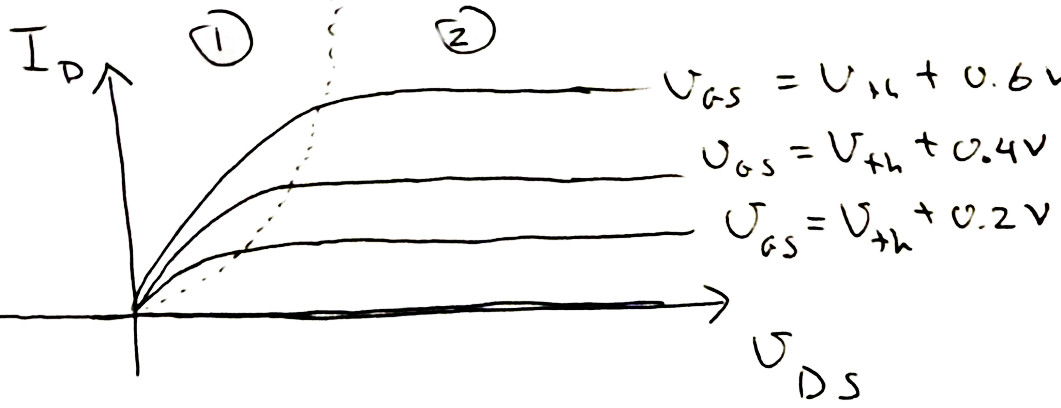
\includegraphics[width=0.8\linewidth]{figures/NMOS-IV}
  \caption{I-V characteristic of an \textsc{nmos} transistor at different values of \(v_\text{GS}\).}
  \label{figure:lec2-NMOS-IV}
\end{figure}
\autoref{figure:lec2-NMOS-IV} depicts several current-voltage characteristics of an \text{nmos}, parameterized by \(v_\text{GS}\).
There's a lot happening on this graph in both the vertical and horizontal directions.
Here's a self-guided tour:
\begin{itemize}
  \item Notice the horizontal line lying along the positive
  \(v_\text{DS}\)-axis.
  This is the plot of the I-V characteristic when
  \(v_\text{GS} < v_\text{t,n}\), where
  \(v_\text{t,n} > 0\)
  is the threshold voltage for an \textsc{nmos} transistor.
  The current-voltage characteristic is \(I=0\),
  the transistor is behaving as a current source corresponding to zero current%
  ---in other words, it's an open circuit.
  The transistor is ``off.''\,\footnote{English semantics for ``on'' and ``off'' in circuits can be counterintuitive. An open circuit/switch is off, and vice versa.}
  \item
  Notice that three I-V curves, parameterized
  by how much \(v_\text{GS}\) exceeds \(v_{t,n}\),
  lie above the line \(I = 0\).
  % \(v_\text{GS} = v_\text{t,n} + 0.2\unit{V}\),
  % \(v_\text{GS} = v_\text{t,n} + 0.4\unit{V}\),
  % and
  % \(v_\text{GS} = v_\text{t,n} + 0.4\unit{V}\).
  Each of them is intersected by what looks like the eastern half of
  a dotted upward-facing parabola rising
  from the origin.
  This parabola divides the quadrant into two regions, one left and one right.
  The left region is called region 1; the right region is called region 2.
  \item
  Focus on region 1, which is called the Linear Region.
  Notice that in region 1 near the origin, \(I_\text{D}\) and \(v_\text{DS}\) are proportional for every value of \(v_\text{GS}\).
  The slope \(G = I_{D} / v_\text{DS}\) increases for higher values of
  \(v_\text{GS}\).
  This means that the D-S resistance \(R = G^{-1}\) transitions from
  \(\infty\) to a finite (perhaps small) value as
  \(v_{GS}\) increases past \(v_{t,n}\).
  A resistor that can alternate between finite and infinite resistance
  is called a switch: in the Linear Region the transistor is a voltage-controlled switch.
  \item
  Focus on region 2, which is called Saturation,
  Here the \(I_{D}\) increases only very weakly
  as \(v_\text{DS}\) increases.%
  % \footnote{Actually this model is somewhat idealistic.
  % In fact \(I_\text{D}\) is very weakly increasing in \(v_\text{DS}\).}
  For a given \(V_{DS}\),
  \(I_\text{D}\) increases with increasing \(v_\text{GS}\):
  the transistor behaves approximately as a voltage-controlled current source!
\end{itemize}
These characteristics are summarized in \autoref{figure:lec2-NMOS-regime-table}.
Regions 0 and 1 can be used to implement a switch.
Region 2 is used for analog electronics---dependent sources,
  amplifiers, etc.

\begin{figure}
  \centering
  \begin{tabular}{lllll}
    region \# & on/off? &
    \(v_\text{GS}\) predicate & \(v_\text{DS}\) predicate
    & name\\\hline
    0 & off & \(v_\text{GS} < v_{t,n}\) & any & \\
    1 & on & \(v_\text{GS} > v_{t,n}\) & low & ``linear region''\\
    2 & on & \(v_\text{GS} > v_{t,n}\) & high & ``saturation''
  \end{tabular}
  \caption{Regions of an \textsc{nmos} I-V characteristic.}
  \label{figure:lec2-NMOS-regime-table}
\end{figure}

\subsection{\textsc{pmos} transistors: opposite of \textsc{nmos}}
\begin{figure}
  \centering
  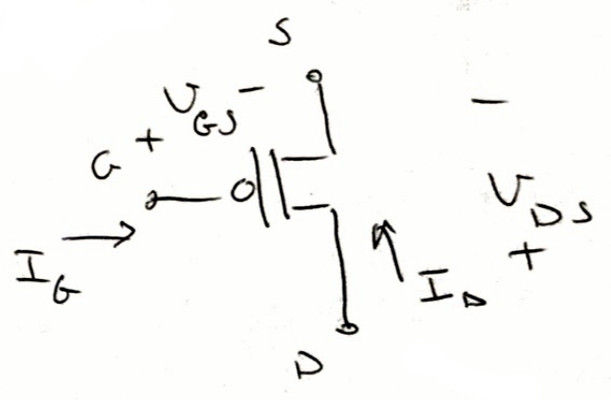
\includegraphics[width=0.5\linewidth]{figures/PMOS-currents-voltages}
  \caption{Currents and voltages labeled on a \textsc{pmos} transistor.}
  \label{figure:lec2-PMOS}
\end{figure}
\begin{figure}
  \centering
  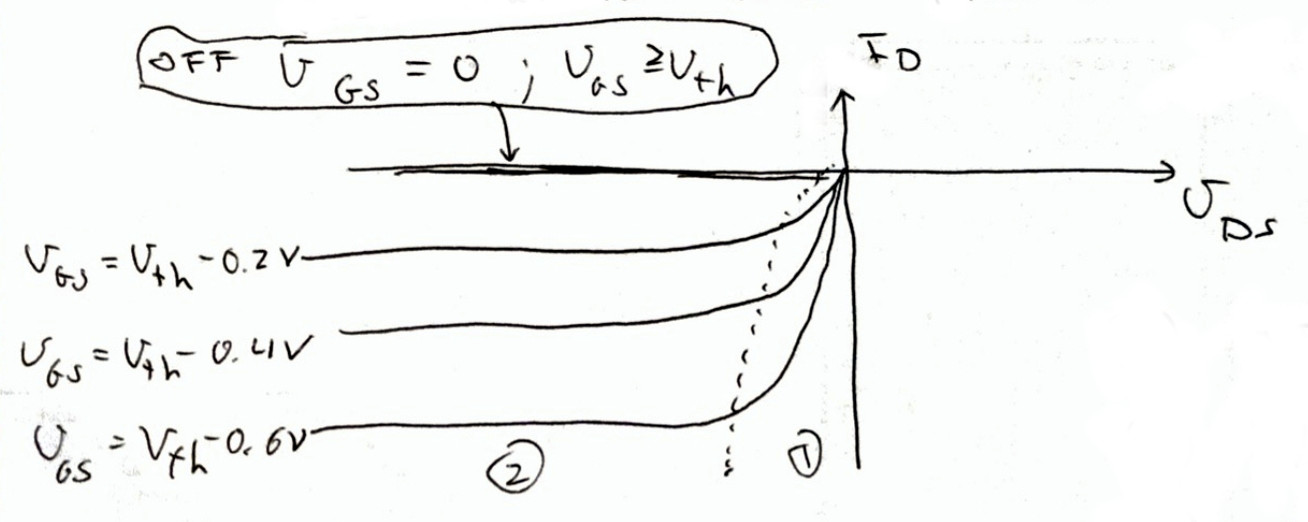
\includegraphics[width=\linewidth]{figures/PMOS-IV}
  \caption{I-V characteristic of a \textsc{PMOS} transistor at different values of \(v_\text{GS}\).}
  \label{figure:lec2-PMOS-IV}
\end{figure}
Another kind of \textsc{mosfet} is the \textsc{pmos}.
They have a similar construction as \textsc{nmos} transistors, but their
behavior is opposite, and for the ``on'' condition of \(V_\text{GS} < V_\text{t,p}\), \(V_\text{t,p} < 0\).
\autoref{figure:lec2-PMOS} and \autoref{figure:lec2-PMOS-IV}
are the counterparts of \autoref{figure:lec2-NMOS} and
\autoref{figure:lec2-NMOS-IV}, respectively.

For most of this class, we'll use more idealized models
of these transistors in digital logic settings.
In the voltage-controlled switch perspective,
\textsc{nmos} transistors open at lower voltages and close at higher voltages,
and \textsc{pmos} transistors close at lower voltages and open at high ones.

\section{An \textsc{nmos} inverter}
One building block we need to understand digital logic is the \emph{inverter},
which is a circuit that outputs a high voltage when its input is a low
voltage, and vice versa.
The high voltage represents a digital value of 1 (true), and the low voltage represents a digital value of 0 (false).

It's possible to build an inverter using an \textsc{nmos} transistor,
as shown in \autoref{figure:lec2-NMOS-inverter}.
The high voltage is called \(V_\text{DD}\), which stands for
the voltage supplied by the high power rail,
and in this example has a value of 1 volt.%
\footnote{For obscure historical reasons.}
In this example, our reference voltage will be ground---0 volts.

\begin{figure}
  \centering
  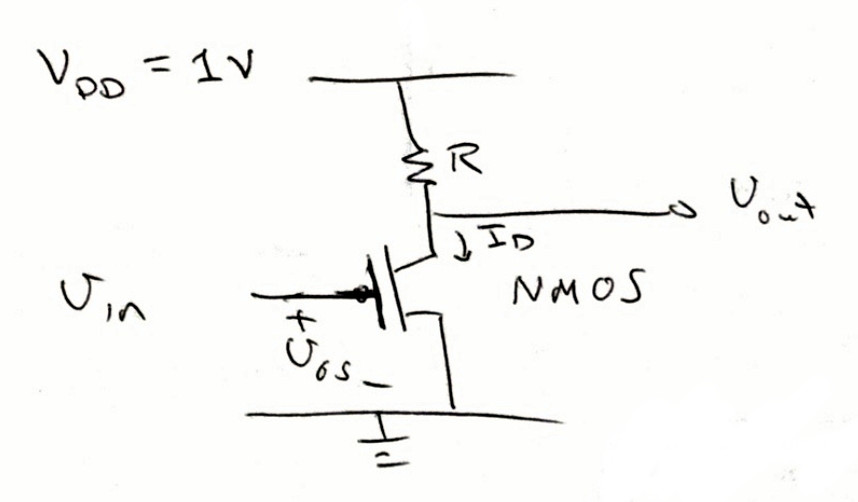
\includegraphics[width=0.75\linewidth]{figures/NMOS-inverter}
  \caption{A inverter built using an \textsc{nmos} transistor.}
  \label{figure:lec2-NMOS-inverter}
\end{figure}

\subsection{Analysis}
\begin{itemize}
\item
(Case \(v_\text{in} = 0\))
The transistor, as a switch, is off.
As a result, the terminal \(v_\text{out}\)
is connected directly to \(V_\text{DD}\) by a resistor.
Because no current flows into the voltage terminal,
by Ohm's law there can be no voltage drop across the resistor.
Therefore \(v_\text{out} = V_\text{DD}\).

\item
(Case \(v_\text{in} = V_\text{DD}\))
The transistor, as a switch, is on. The terminal \(v_\text{out}\) has a short to ground, so \(v_\text{out} = 0\).
\end{itemize}

\autoref{figure:lec2-inverter-truth-table} shows
the truth table of this circuit and verifies that this circuit is indeed
an inverter.

\begin{figure}
  \centering
  \begin{tabular}{ll}
    \(v_\text{in}\) & \(v_\text{out}\) \\\hline
    0 & \(V_\text{DD}\)\\
    \(V_\text{DD}\) & 0
  \end{tabular}
  \caption{Truth table of the \textsc{nmos} inverter.}
  \label{figure:lec2-inverter-truth-table}
\end{figure}

\subsection{Power consumption}
When \(v_\text{in} = 0\), the circuit consumes no power, as we have established that there is no current through the resistor between \(V_\text{DD}\) and \(v_\text{out}\).
When \(v_\text{in} = V_\text{DD}\), there is a path from \(V_\text{DD}\) through the resistor, then the transistor, to ground.
The circuit consumes power \(VI = {V_\text{DD}^2}/{R}\).
While this might not necessarily be a lot, in computing applications with countless transistors, it adds up, and moving heat away from a dense circuit poses engineering challenges.
Dense digital circuits were made possible by the discovery of the CMOS inverter architecture, which avoids a path from \(V_\text{DD}\) to ground.

\section{A \textsc{cmos} inverter}
\begin{figure}
  \centering
  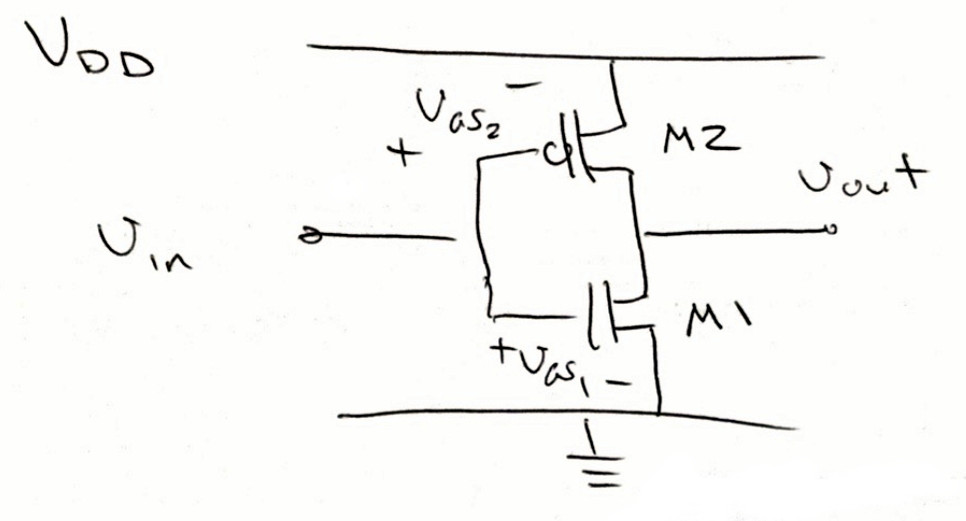
\includegraphics[width=0.75\linewidth]{figures/CMOS-inverter}
  \caption{A inverter built using the \textsc{cmos} design..}
  \label{figure:lec2-CMOS-inverter}
\end{figure}

\autoref{figure:lec2-CMOS-inverter} shows an inverter circuit that exemplifies the \textsc{\em cmos} design strategy of using \textsc{pmos} and \textsc{nmos} transistors together.

\begin{figure}
  \centering
  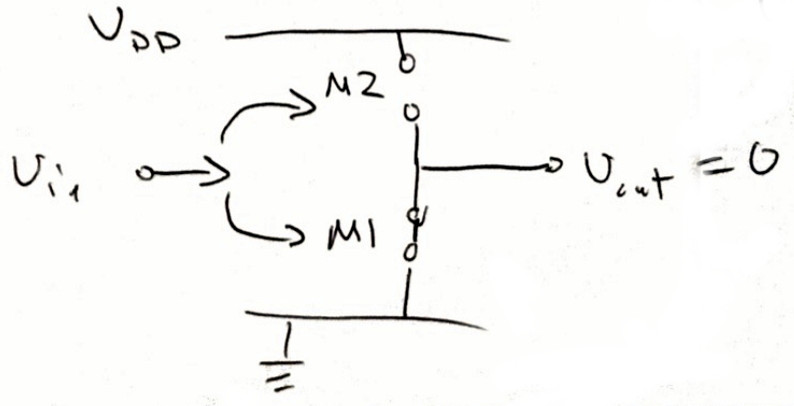
\includegraphics[width=0.75\linewidth]{figures/CMOS-case}
  \caption{Equivalent circuit of \autoref{figure:lec2-CMOS-inverter}
  when \(v_\text{in} = V_\text{DD}\).}
  \label{figure:lec2-CMOS-case}
\end{figure}

\subsection{Analysis}
\begin{itemize}
  \item
  (Case \(v_\text{in} = V_\text{DD}\))
  \begin{itemize}
    \item
    The \textsc{pmos} having as its source \(V_\text{DD}\) and \(v_\text{out}\) as its drain
    \(V_\text{GS,1} = 0\), which is higher than \(V_\text{t,p}\).
    Therefore there is no path from \(V_\text{DD}\) to \(v_\text{out}\).
    \item
    The \textsc{nmos} having \(v_\text{out}\) as its drain and ground as its source has \(V_\text{GS,2}= V_\text{DD}\),
    which is higher than \(V_\text{t,n}\).
    Therefore, due to the terminal's short to ground, \(v_\text{out} = 0\).
  \end{itemize}
  The equivalent circuit once the switch model has been applied is shown in  \autoref{figure:lec2-CMOS-case}.

  \item
  (Case \(v_\text{in} = 0\))
  \begin{itemize}
      \item
      The \textsc{pmos}, having \(V_\text{GS,1} = -V_\text{DD} < V_\text{t,p}\), turns on.
      \item
      The \textsc{nmos}, having \(V_\text{GS,2} = 0 < V_\text{t,n}\), turns off.
  \end{itemize}
  Therefore \(V_\text{out} = V_\text{DD}\).
\end{itemize}

\subsection{Power consumption}
All currents are zero in this model, so no power is consumed.

\section{A \textsc{cmos} inverter chain with capacitance}
\begin{figure}
  \centering
  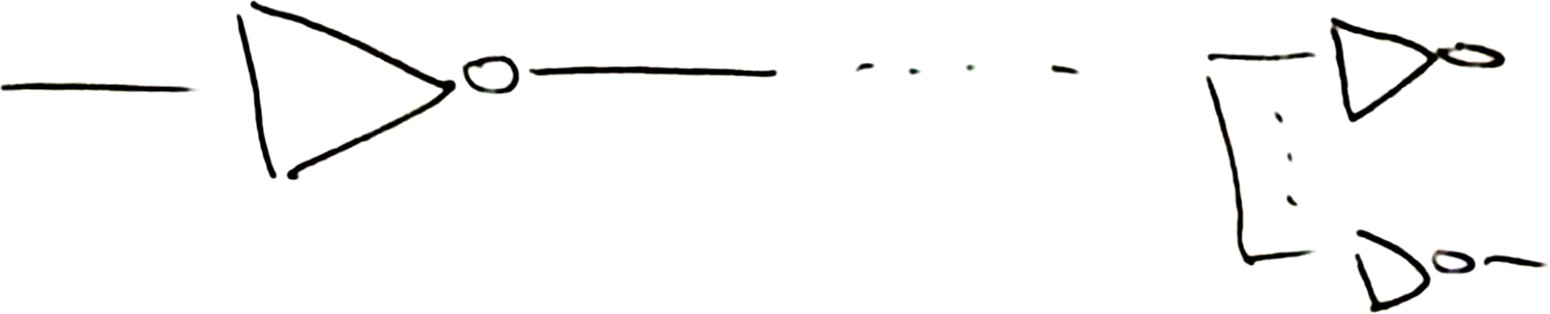
\includegraphics[width=0.75\linewidth]{figures/inverter-chain}
  \caption{A chain of inverters, which is kind of similar to a computer.}
  \label{figure:lec2-inverter-chain}
\end{figure}
Contrary to our last conclusion, inverters in real electronics certainly do consume some power.
We'll pretend digital circuits are chains of inverters (\autoref{figure:lec2-inverter-chain})---although this model won't teach you how to build a computer, it is close enough to real \textsc{cmos} networks to illustrate when and where power is expended.

We will concentrate our analysis on just one stage of the \textsc{cmos} inverter chain.
A single inverter is shown in \autoref{figure:lec2-CMOS-cap},
with a capacitor between \(v_\text{out}\) and ground to model the
next stage's load.
\begin{figure}
  \centering
  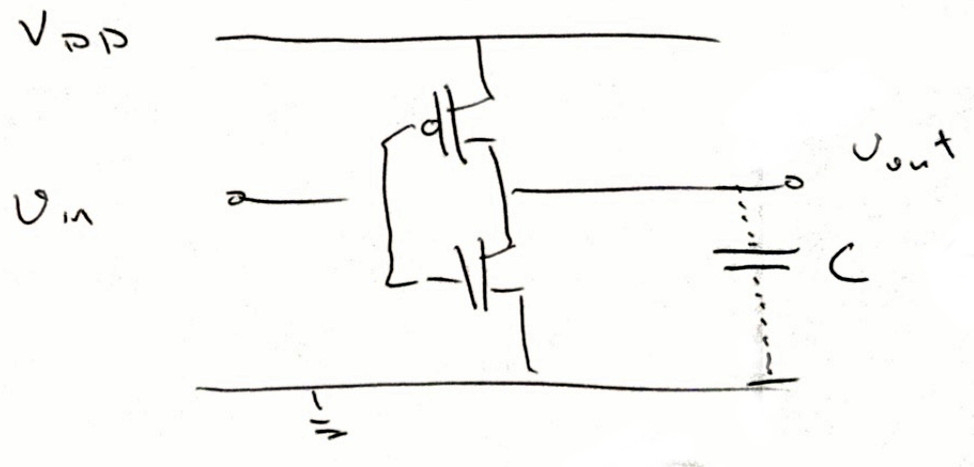
\includegraphics[width=0.75\linewidth]{figures/CMOS-inverter-with-out-cap}
  \caption{An inverter taken from a chain with a capacitor modeling the next stage.}
  \label{figure:lec2-CMOS-cap}
\end{figure}
\autoref{figure:lec2-CMOS-cap-1} shows the equivalent circuit when the output of this inverter settles at \(V_\text{DD}\).
\begin{figure}
  \centering
  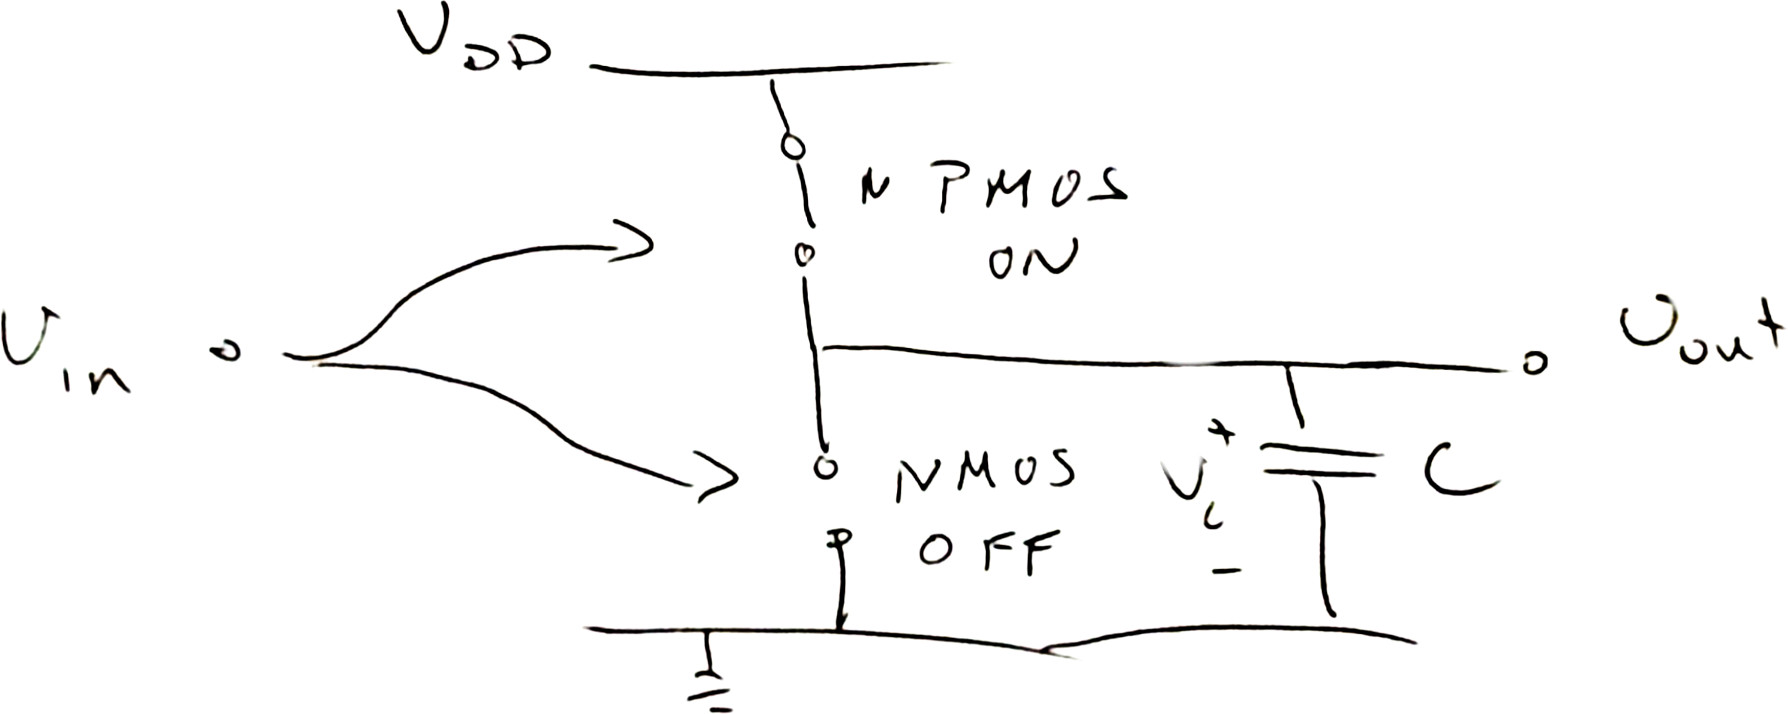
\includegraphics[width=0.75\linewidth]{figures/CMOS-cap-1}
  \caption{An inverter outputting \(V_\text{DD}\) with load capacitor.}
  \label{figure:lec2-CMOS-cap-1}
\end{figure}

\subsection{Potential energy in a capacitor}
\begin{figure}
  \centering
  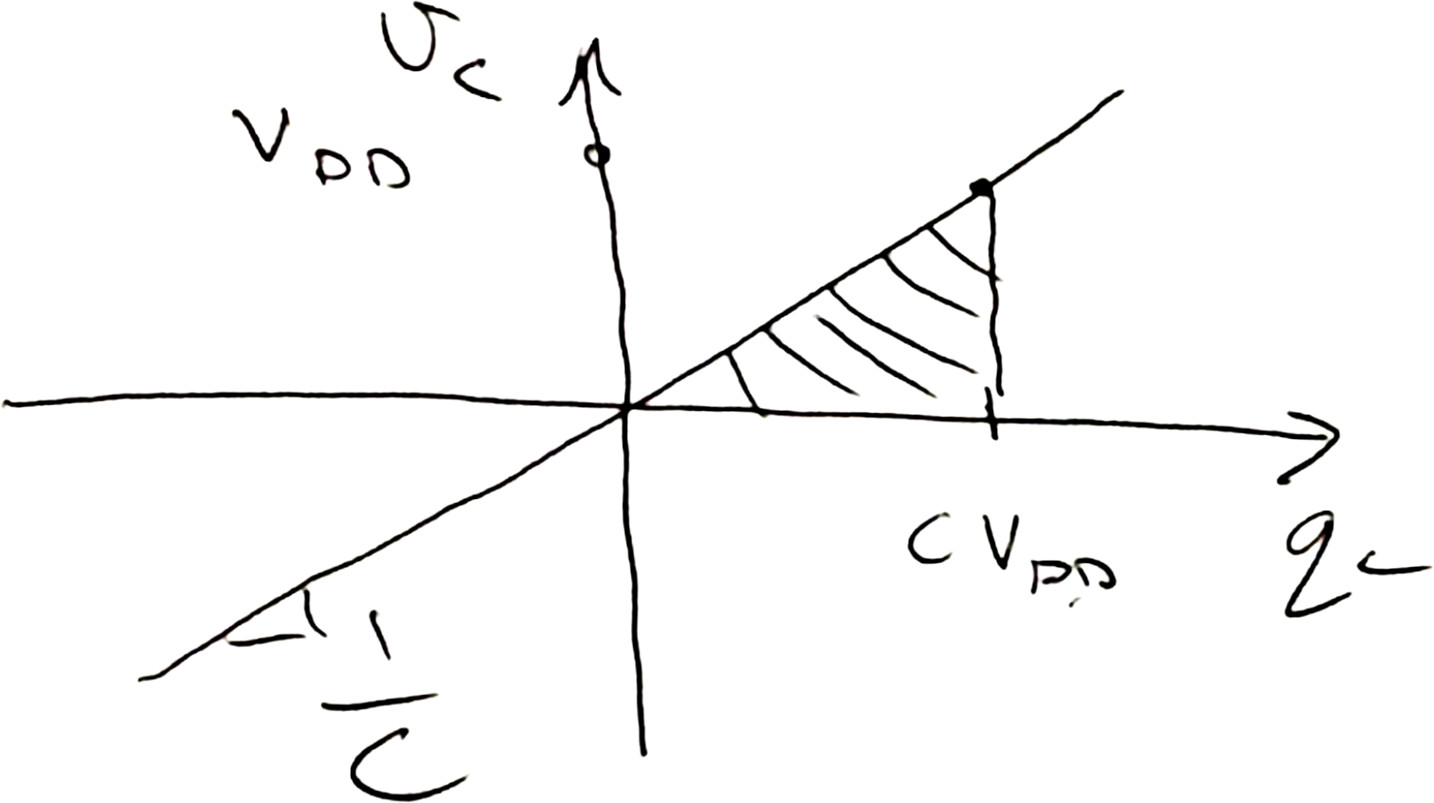
\includegraphics[width=0.75\linewidth]{figures/cap-energy-integral}
  \caption{Energy stored in a capacitor can be computed by an integral under the \(V = Q/C\) curve.}
  \label{figure:lec2-cap-energy-integral}
\end{figure}
The energy stored in the capacitor when it has voltage \(V_\text{DD}\) is given by the formula
\begin{align}
  E_\text{cap}
  &= \frac{1}{2} CV_\text{DD}^2,
\end{align}
which can be derived by using the facts that 1) that voltage is energy per unit charge and 2) a capacitor obeys \(Q = CV\), and integrating through the total charge stored in the capacitor: \(\int_0^{CV_\text{DD}} v_C \dif q\) (\autoref{figure:lec2-cap-energy-integral}).

\begin{figure}
  \centering
  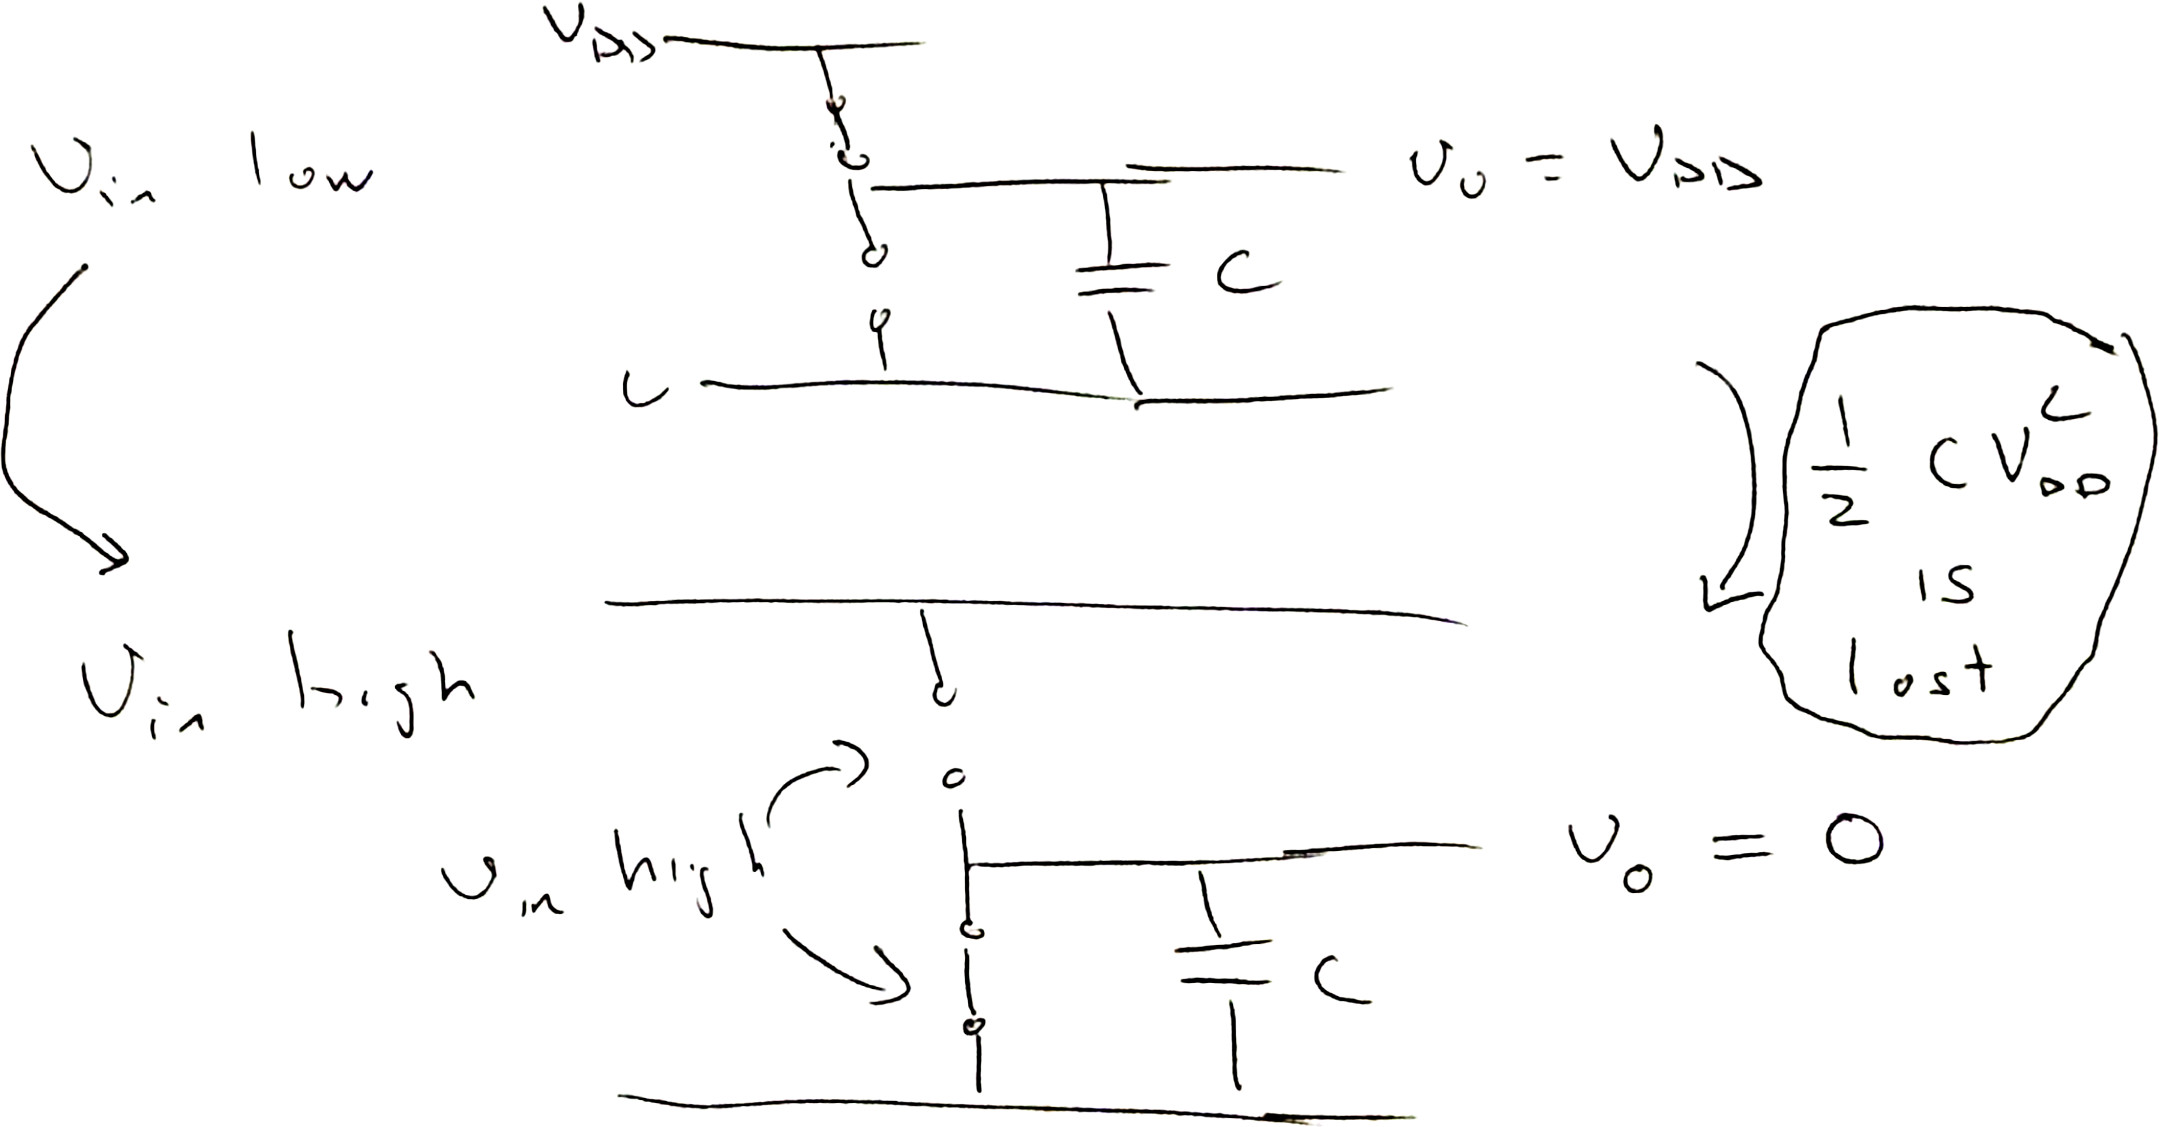
\includegraphics[width=1\linewidth]{figures/cap-discharge-energy}
  \caption{\textsc{cmos} load capacitor forced from voltage \(V_\text{DD}\) to \(0\).}
  \label{figure:lec2-cap-discharge-energy}
\end{figure}
When the inverter's input changes from low to high, the output must change from \(V_\text{DD}\) to \(0\) (\autoref{figure:lec2-cap-discharge-energy}).
That means that the load capacitor must discharge fully, burning \(\frac{1}{2}CV_\text{DD}^2\) of potential energy as heat.

\subsection{Total energy supplied}
Even though the capacitor only stores and discharges
\(\frac{1}{2}CV_\text{DD}^2\),
an up-down cycle costs \(CV_\text{DD}^2\).
This is because the voltage source must offer \(Q = CV_\text{DD}\) of charge
at \(V_\text{DD}\) energy per unit charge.
Where does this go? Let's follow the energy as the output changes from 0 to 1 and back to 0.
\begin{enumerate}
  \item (\(q_C = 0\), \(v_C = 0\))
  \item Voltage source loads \(CV_\text{DD}\) of charge at \(V_\text{DD}\) energy per unit charge, at a total expense of \(CV_\text{DD}^2\).
  Half of its energy output is burned by ``parasitic'' resistance en route to the capacitor, and the other half is stored in the capacitor.
  \item (\(q_C = CV_\text{DD}\), \(v_C = V_\text{DD}\))
  \item Transistors toggle, and the capacitor drains, generating \(\frac{1}{2} CV_\text{DD}^2\) of heat on the pull-down circuit.
  \item (\(q_C = 0\), \(v_C = 0\))
\end{enumerate}

\subsection{Where does the energy in a device go?}
With reference to our chain-of-inverters model,
power consumption in digital devices is mainly explained by three phenomena:
\begin{itemize}
  \item If the inverter flips every cycle at a clock speed of \(f_s\),
  the circuit will burn \(f_sCV_\text{DD}^2\) charging its capacitors.
  \item Leakage: a transistor that's ``off'' isn't 100\% off, and a small amount of current flows and burns some energy.
  \item Short-circuit current (smaller): when the input is flipping between 0 and 1, there's a very short instant during which both transistors may be \emph{on}, and some current flows through the momentary \(V_\text{DD}\)-ground short.
\end{itemize}
